%&latex

%&latex
\documentclass[notes=show]{beamer}
%%%%%%%%%%%%%%%%%%%%%%%%%%%%%%%%%%%%%%%%%%%%%%%%%%%%%%%%%%%%%%%%%%%%%%%%%%%%%%%%%%%%%%%%%%%%%%%%%%%%%%%%%%%%%%%%%%%%%%%%%%%%%%%%%%%%%%%%%%%%%%%%%%%%%%%%%%%%%%%%%%%%%%%%%%%%%%%%%%%%%%%%%%%%%%%%%%%%%%%%%%%%%%%%%%%%%%%%%%%%%%%%%%%%%%%%%%%%%%%%%%%%%%%%%%%%
\usepackage{amssymb}
\usepackage{mathpazo}
\usepackage{hyperref}
\usepackage{multimedia}
\usepackage{graphicx}
\usepackage{amssymb}
%%\usepackage[utf8]{inputenc}
%\usecolortheme[named=black]{structure}
%\usetheme[height=10mm]{Rochester}
\usetheme{CambridgeUS}
%\input{tcilatex}
\begin{document}

\title[]{Del 4 - Applikasjon: Krisen i eurosonen}
\author[]{J\o rn Inge Halvorsen \inst{1}
\\Merk: Som nevnt under forelesningen, vil dere ikke bli spurt om dette p\aa \ eksamen. Men presentasjonen viser likevel hvor relevant temaene vi har snakket om i kurset kan v\ae re i praktisk politikk. }
\institute[JIH]{Presentasjon: Universitetet i \AA s }
\date[]{28. November, 2013}

\maketitle
\section{Bakgrunn}
\begin{frame}
\frametitle{Hvorfor opprettelsen av en felles valuta i europa?}
\begin{itemize}
\item Fjerne transaksjonskostnader
\item Forbedre konkurransen ved \aa \ gj\o re det lettere \aa sammenlikne priser
\item Redusere Bundesbanks innflytelse
\item Bidrag til \aa \ skape en tettere integrasjon mellom europeiske land 
\end{itemize}
\end{frame}
\begin{frame}
\frametitle{Hvs skjedde under og etter innf\o ringen av euroen?}
\begin{itemize}
\item De forskjellige landenes rentespread mot tyske statsobligasjoner ble eliminert
\begin{figure}[h]
\caption{Lange renter p\aa \ statsobligasjoner med 10-\aa rs l\o petid}
\begin{center}
\includegraphics{spreadeuro.png}
\end{center}
\end{figure}
\end{itemize}
\begin{itemize}
\item Dette ga st\o tet til en kredittfinansiert h\o ykonjunktur for landene i s\o r, spesielt for Portugal, Spania, Irland, (Italia) og Hellas (PI(I)GS-landene)
\end{itemize}
\end{frame}
\begin{frame}
\frametitle{}
\begin{itemize}
\item Oppl\aa ningen skjedde b\aa de i privat (\o kt  C) og offentlig sektor (\o kt G).
\item L\o nninger og priser steg kombinert med en sterk grad av missallokering(?) av resssurser i \o konomien
\end{itemize}
\begin{equation*}
C\uparrow / G\uparrow  \Rightarrow Y \uparrow  \Rightarrow P(W)\Rightarrow P^e(W) 
\uparrow  \Rightarrow NX \downarrow 
\end{equation*}
\begin{itemize}
\item P\aa \ utenriksregnskapet til landene i s\o r eurosonen ga dette seg utslag ved
\begin{equation*}
 DRI\downarrow +KRI \uparrow=\Delta TR \approx 0
\end{equation*}
\end{itemize}
\end{frame}
\begin{frame}
\frametitle{Finanskrisen i 2008 og situasjonen i dag}
\begin{itemize}
\item Som en f\o lge av finanskrisen i USA\ i 2008, begynte utenlandske investorer \aa \ forlange en risikopremie for \aa \ investere i landene i s\o r
\item Den privare gjeldskrisen bidra for mange land ogs\aa \ til en statlig gjeldskrise 
\begin{figure}[h]
\caption{Gjeld som andel av BNP}
\begin{center}
\includegraphics{gjeldbnp.png}
\end{center}
\end{figure}
\end{itemize}
\end{frame}
\begin{frame}
\frametitle{}
\begin{itemize}
\item Men forel\o pig f\aa\  tegn til deflasjon? 
\begin{equation*}
C\downarrow / G\downarrow  \Rightarrow Y \downarrow  \Rightarrow P(W) \approx  P^e(W) \approx 0 
\end{equation*}
\item Svaret p\aa\ hvorfor viser seg \aa \ v\ae re reflektert i balansen til det elektroniske betalingssystemet TARGET(2), som benyttes av alle de nasjonale sentralbankene som inng\aa r i eurosonen
\end{itemize}
\end{frame}
\begin{frame}
\frametitle{}
\begin{figure}[h]
\caption{Fordringer (+) og gjeld (-) p\aa \ TARGET-balansen}
\begin{center}
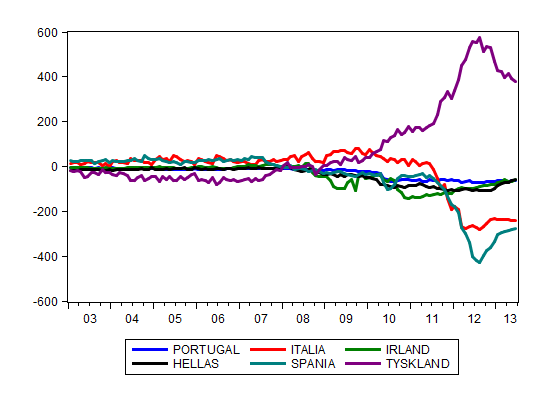
\includegraphics{targetbalanse.png}
\end{center}
\end{figure}
\end{frame}
\begin{frame}
\frametitle{}
\begin{itemize}
\item Utenriksregnskapet under fast kurs\\
\begin{eqnarray*}
 \Delta RES= DR+KR \\ 
\end{eqnarray*}
Hvor $\Delta RES$ er endring p\aa \ balansen i sentralbankens valutareserver
\item Innad i eurosonen \\
\begin{eqnarray*}
\Delta TR=(DR-DRV)+(KR-KRV) = DRI+KRI
\end{eqnarray*}
Hvor $\Delta TR$ er endring p\aa TARGET-balansen i sentralbankens valutareserver
\item Sinn og Wollmershausen (2011) tolker ubalansen som en klassisk betalingskrise for utenrikshandelen mellom land (eks. Bretton-Woods sammarbeidet) 
\end{itemize}
\end{frame}
\section{Bretton-Woods som paralell}
\begin{frame}
\frametitle{Hva var Bretton-Woods sammarbeidet? }
\begin{itemize}
\item Internasjonal pengepolitisk avtale i etterkant av den andre verdenskrig mellom USA og mange av dens allierte
\item USA forpliktet seg ovenfor de andre lands sentralbankner \aa \ holde en fast innl\o sningskurs for verdien av dollar mot gull\item De andre landene skulle s\o rge for at sin valuta stod i et fast forhold til dollaren (+/- prosent)
\item Ingen restriksjoner p\aa \ landenes pengemengdevekst
\end{itemize}
\end{frame}

\begin{frame}
\frametitle{}
\begin{figure}[h]
\caption{Penger utenfor landets grenser under Bretton Woods-systemet. For�rsaket her av en \o kning i basispenger.}
\begin{center}
\includegraphics[scale=0.70]{balanse_dr_bw.png}
\end{center}
\end{figure}
\end{frame}
\begin{frame}
\frametitle{Oppl\o sningen av Bretton-Woods sammarbeidet}
\begin{itemize}
\item Pengemengdeveksten var i en lengre periode mye sterke i USA enn blant de andre landene som inngikk  i sammarbeidet
\item Store dollarreserver akkumulerte seg derfor opp i de andre landenes nasjonale sentralbanker
\item Det ble etterhvert klart at dollarreservene kunne anses som noen troverdige fordringer p\aa gull
\item President de Gaulle i Frankrike fremsatte derfor etterhvert en trussel om \aa \ omgj\o re de franske dollarreservene til gull 
\item Nixon tilsvar i 1971, suspendere innl\o snings muligheten og dermed oppl\o se  hele valutasammarbeidet
\end{itemize}
\end{frame}
\section{TARGET-ubalanser}
\begin{frame}
\frametitle{Forskjeller mellom Bretton-Woods og euro-sammarbeidet}
\begin{itemize}
\item Mellom landene i eurosonen er �fastkursforholdet� 1:1 
\item I dag skjer for det meste pengetransaksjoner elektronisk (TARGET 2-systemet). \item Fordringer p\aa \ TARGET-balansen er uten formelle innl\o sningsmuligheter \item En \o kning i basispengemengden klareres ved at ESB endrer TARGET-balansen til de nasjonale sentralbankene.   
\item Det er ESB-styret som har ut\o vende makt til \aa \ endre basispengemengden
\end{itemize}
\end{frame}

\begin{frame}
\frametitle{}
\begin{figure}[h]
\caption{Penger utenfor landets grenser i eursonen. For\aa rsaket her av en \o kning i basispengemengden.}
\begin{center}
\includegraphics[scale=0.70]{balanse_dr_euro.png}
\end{center}
\end{figure}
\end{frame}
\begin{frame}
\frametitle{}
\begin{figure}[h]
\caption{Penger utenfor landets grenser i eursonen. For\aa rsaket her av endrede innskuddspreferanser.}
\begin{center}
\includegraphics[scale=0.70]{balanse_kr_euro.png}
\end{center}
\end{figure}
\end{frame}
\begin{frame}
\frametitle{ESBs pengepolitkk i etterkant av finanskrisen}
\begin{itemize}
\item Fra oktober 2008 til mai 2009 ble rente p\aa\ refinansieringsl\aa n redusert fra 4,25 prosent til 1 prosent
\item Krav til sikkerhet for refinansieringsl\aa n ble ogs\aa redusert, fra en rating A- til BBB
\item Hellas, Ireland og Portugal ble tilbudt l\aa n uten krav til sikkerhet (ELA-l\aa n)   
\end{itemize}
\end{frame}
\begin{frame}
\frametitle{}
\begin{figure}[h]
\caption{Utviklingen i Target-gjelden og driftsbalansen (positivt tall er underskudd) for PIGS-landene totalt. Bel\o pene er i milliarder av euro }
\begin{center}
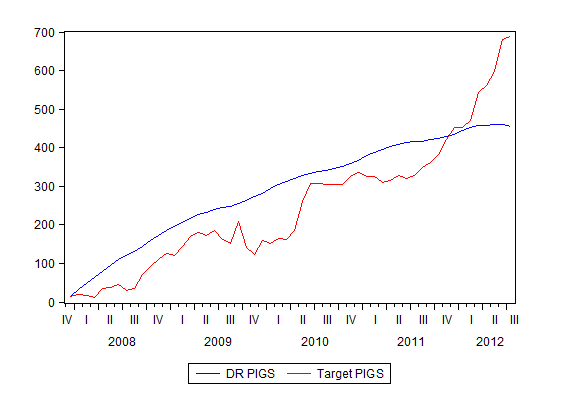
\includegraphics{target_bal_piigs.png}
\end{center}
\end{figure}
\begin{multline}
\sum_{1=2008}^{T=2013} \Delta TR= \ \Delta TR_{1}+\Delta TR_{2}+...+\Delta TR_{T}=\\(DRI_{1}-KRI_{1})+(DRI_{2}-KRI_{2})+...+(DRI_{T}-KRI_{T})
\end{multline}

\end{frame}
\begin{frame}
\frametitle{}
\begin{figure}[h]
\caption{Utviklingen i Target gjelden og driftsbalansen (positivt tall er underskudd) for Portugal, Ireland, Hellas, Spania og Italia enkeltvis. Bel\o pene er i milliarder av euro}
\begin{center}
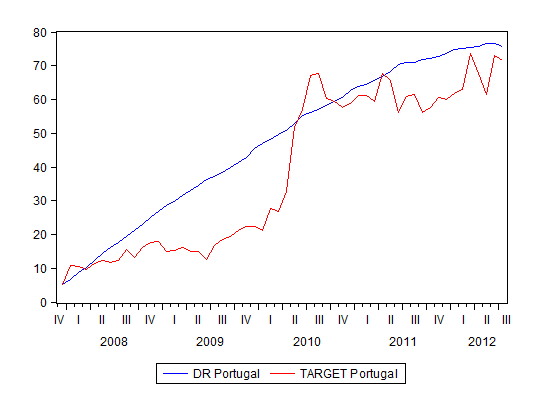
\includegraphics[scale=0.70]{target_bal_portugal.png}
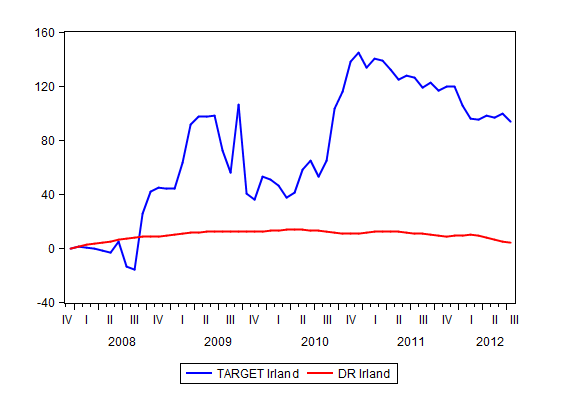
\includegraphics[scale=0.70]{target_bal_irland.png}
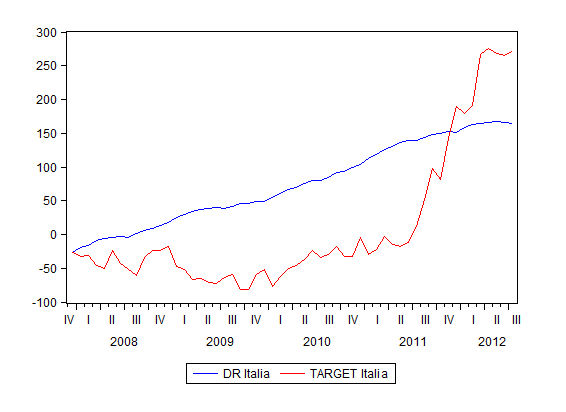
\includegraphics[scale=0.70]{target_bal_italia.png}\\
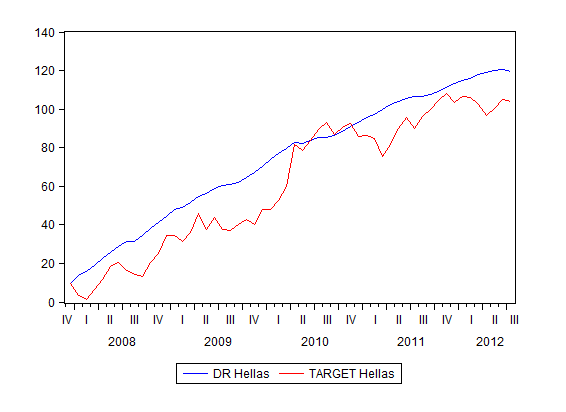
\includegraphics[scale=0.70]{target_bal_hellas.png}
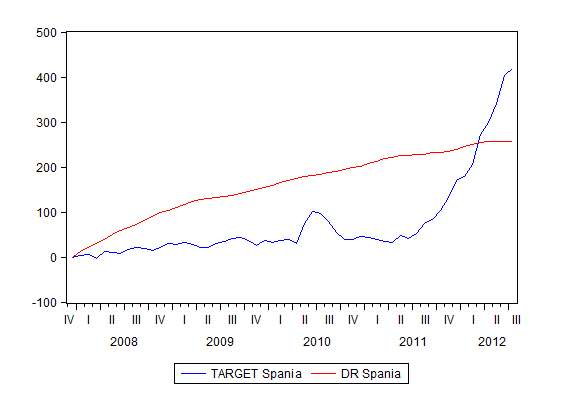
\includegraphics[scale=0.70]{target_bal_spania.png}
\end{center}
\end{figure}
\end{frame}
\begin{frame}
\frametitle{Hva ville konsekvensene ha v\ae rt dersom ESB ikke hadde tilbudt forretningsbankene refinansieringsl\aa n under markedspris? }
\begin{itemize}
\item Spesialtilfelle 1: Med uendret nettokapitalimport i perioden
\begin{multline*}
\sum_{1}^{T} \Delta TR = \Delta TR_{1}+\Delta TR_{2}+...+\Delta TR_{T}= \\ (DRI_{1}+DRI_{2}+...+DRI_{T})
\end{multline*}
Gitt at $\sum_{1}^{T} \Delta TR=0$ $\Rightarrow$ $(DRI_{1}+DRI_{2}+...+DRI_{T})=0$
\end{itemize}
Driftsbalansen ville ha v\ae rt i balanse: $\Rightarrow Y \downarrow$ $\Rightarrow P(W) \downarrow   \Rightarrow P^e(W)\downarrow$
\end{frame}
\begin{itemize}
\item Spesialtilfelle 2: Med uendret driftsbalanse i perioden
\begin{multline}
\sum_{1}^{T} \Delta TR = \Delta TR_{1}+\Delta TR_{2}+...+\Delta TR_{T}= \\ (KRI_{1}+KRI_{2}+...+KRI_{T})
\end{multline}
Gitt at $\sum_{1}^{T} \Delta TR=0$ $\Rightarrow$ $(KRI_{1}+KRI_{2}+...+KRI_{T})=0$
\end{itemize}
Uendret kapitalflukt: $\Rightarrow$ Gjelden blitt misligholdt, private investorer vil m\aa te ta store tap\\
\begin{frame}
\frametitle{}
\begin{center}
Generelt har ECBs pengepolitikk bidratt til finansielle stabilitet, men konsekvensen av dette har v\ae rt  
\begin{enumerate}
\item Satt til side de selvkorrigerende mekanismene som gjelder for utenrikshandelen mellom land
\item Storstilt grad klart \aa \ overf\o re risiko fra investorer til de nasjonale sentralbankene
\end{enumerate}
\end{center}
Kan forventninger om en slik politikk forklare hvorfor rentespreaden forsvant i 2001? Hvis ja, $\Rightarrow $ hele systemet er ustabilt
\end{frame}
\section{Veien videre?}
\begin{frame}
\frametitle{Veien videre?}
\begin{enumerate}
\item Tilbake til markedene\\
$\Rightarrow $ Kapitalflukt og l\o p p\aa bankene(?)
\item \O kt inflasjon i nord \\
$\Rightarrow$ Finanspolitikken m\aa \ ta sv\ae rt mye av jobben, siden renta allerede ligger n\ae r null
\item Sosialisering av bank- og statsgjeld (Eurobonds, OMT og bankunion)
$\Rightarrow $ Risikopremien reduseres\\
$\Rightarrow $ Allokering av kapital blir i stor grad en jobb utf\o rt av byr\aa krater og ikke av markedet\\  
$\Rightarrow $ Ledighetsproblemet vil st\aa ul\o st i lang, lang, tid... 
\end{enumerate}
\end{frame}
\end{document}
